\subsection{AIM-9 SIDEWINDER}
\label{subsec:aim9}
\begin{figure}[htbp]
    \centering
    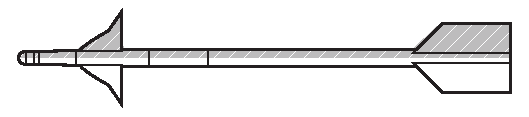
\includegraphics[
            width = 0.8\textwidth,
    ]{diagrams/weap/weap_aa_aim9_overview.pdf}
    % TODO: labels? some kind of flavor stuff?
    \caption{AIM-9 Sidewinder}
\end{figure}

\begin{tcoloritemize}
    \blueitem{AIM-9 \break Sidewinder}{
    Short-range, fire-and-forget ``dogfight'' missile. First entered service in 1956

    \begin{subitemize}
        \item \textbf{Guidance} --- IR-guided (\textbf{Fox 2})
        \item \textbf{Range} --- min: \textasciitilde3000ft, max: \textasciitilde10-20nm
    \end{subitemize}}
    \blueitem{Variants}{
    \begin{subitemize}
        \item \textbf{9M} --- IR-guided, short range, all-aspect
        \item \textbf{9X} --- HOBS (\textbf{H}igh \textbf{O}ff-\textbf{B}ore\textbf{S}ight) capable, thrust-vectored, all-aspect
    \end{subitemize}}
    \blueitem{Acquisition / Cueing Modes}{
    \begin{subitemize}
        \item \textbf{Acquisition with own missile seeker (BORE)} \\
        \hyperref[subsec:aim9:bore]{See \Cref{subsec:aim9:bore}}
        \item \textbf{Seeker cued with HMD LOS (BORE)} \\
        {See \Cref{subsec:aim9:hmcs}}
        \item \textbf{Seeker slaved to radar track LOS (SLAVE)} \\
        \hyperref[subsec:aim9:slave]{See \Cref{subsec:aim9:slave}}
    \end{subitemize}}
    \blueitem{Select AIM-9}{
    Via Dogfight --- AIM-9 \& GUN automatically selected

    \begin{subenumerate}
        \item \textbf{DGFT/MSL OVRD} \dotfill \textbf{DGFT}
        \item \textbf{Selected Weapon (OSB 7)} \dotfill Verify \textbf{9LM / 9X}
    \end{subenumerate}

    Via Missile Override

    \begin{subenumerate}
        \item \textbf{DGFT/MSL OVRD} \dotfill \textbf{OVRD}
        \item \textbf{Selected Weapon (SMS OSB 7)} \dotfill \textbf{9LM / 9X}
    \end{subenumerate}

    Via A-A Master Mode

    \begin{subenumerate}
        \item \textbf{Master Mode} \dotfill \textbf{A-A}
        \item \textbf{Operating Mode (SMS OSB 1)} \dotfill Verify \textbf{AAM}
        \item \textbf{Selected Weapon (SMS OSB 7)} \dotfill \textbf{9LM / 9X}
    \end{subenumerate}
    
    Selected weapon can also be cycled with \textbf{NWS/MSL Step depress (long)}
    }
\end{tcoloritemize}
    
\subsubsection{SMS CONTROLS}

\begin{tcoloritemize}
    \blueitem{SPOT / SCAN}{
    \textbf{OSB 2} controls seeker field of view
    \begin{subitemize}
        \item \textbf{SPOT} --- Narrow, increased detection range
        \item \textbf{SCAN} --- Wide, decreased detection range
    \end{subitemize}}
    \blueitem{Selected Weapon}{
    \textbf{OSB 7} cycles through available A-A weapon types
    
    \medskip
    Selected weapon can also be cycled with \textbf{NWS/MSL Step depress (long)}
    }
    \blueitem{WARM / COOL}{
    \textbf{OSB 8} controls seeker cooling status

    \begin{subitemize}
        \item \textbf{COOL} ---  increases seeker sensitivity, should be set prior to engagement
        \item Set automatically for \textbf{DGFT} \& \textbf{MSL OVRD}
    \end{subitemize}}
    \blueitem{Selected Station}{
    \textbf{OSB 10 / 16} select/cycle available missile pylons
    
    \medskip
    Selected station can also be cycled with \textbf{NWS/MSL Step depress (short)}
    }
    \blueitem{SLAVE / BORE}{
    \textbf{OSB 19} controls seeker line-of-sight

    \begin{subitemize}
        \item \textbf{BORE} --- \hyperref[subsec:aim9:bore]{\textbf{See \Cref{subsec:aim9:bore}}}
        \begin{itemize}
            \item acquisition with own missile seeker
            \item or cued with HMD (if powered)
            \item \textbf{does NOT require FCR}
        \end{itemize}
        \item \textbf{SLAVE} --- \hyperref[subsec:aim9:slave]{\textbf{See \Cref{subsec:aim9:slave}}}
        \begin{itemize}
            \item seeker slaved to radar track LOS
            \item typically via ACM Modes
        \end{itemize}
    \end{subitemize}
    
    Line-of-sight mode can also be cycled with \textbf{Cursor Enable Depress}}
\end{tcoloritemize}

\begin{figure}[htbp]
    \centering
    \begin{tikzpicture}[auto, node distance=10mm, x=1mm, y=1mm, very thick, line cap=round,
        >={Latex[round]}
        ]
        
        \node[] (fig) at (0,0) {
            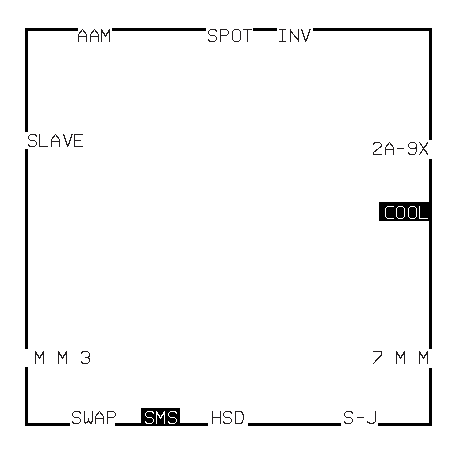
\includegraphics[
                height=75mm,
            ]{mfd/sms/aim9.pdf}
        };

        % Annotations
        \node[lannot] (mode) at ($(fig.west)+(0mm,27mm)$) {Operating \\ mode};
        \draw[->, red] (mode.east) -- ++(10mm, 0mm) -- (-25mm,29mm);

        \node[lannot] (los) at ($(fig.west)+(0mm,14.5mm)$) {LOS mode};
        \draw[->, red] (los.east) -- ++(4mm, 0mm);

        \node[lannot] (lstation) at ($(fig.west)+(0mm,-21mm)$) {Selected station};
        \draw[->, red] (lstation.east) -- ++(4mm, 0mm);

        \node[rannot] (inv) at ($(fig.east)+(0mm,27mm)$) {Inventory};
        \draw[->, red] (inv.west) -- ++(-21mm, 0mm) -- (14mm, 29mm);

        \node[rannot] (sel) at ($(fig.east)+(0mm,13mm)$) {Selected \\ weapon};
        \draw[->, red] (sel.west) -- ++(-4mm, 0mm);

        \node[rannot] (cool) at ($(fig.east)+(0mm,3mm)$) {Cooling \\ status};
        \draw[->, red] (cool.west) -- ++(-4mm, 0mm);

        \node[rannot] (lstation) at ($(fig.east)+(0mm,-21mm)$) {Selected station};
        \draw[->, red] (lstation.west) -- ++(-4mm, 0mm);

        \node[rannot] (sj) at ($(fig.east)+(0mm,-36mm)$) {Selective Jettison};
        \draw[->, red] (sj.west) -- ++(-12.5mm, 0mm) -- ($(fig.south) + (22mm,6mm)$);
    \end{tikzpicture}
    \caption{AIM-9 SMS Page}
    \label{fig:aa_weap:aim9:sms}
\end{figure}

\clearpage

\subsubsection{SYMBOLOGY}
\begin{tcoloritemize}
    \blueitem{MFD Symbology}{Reference \Cref{subsec:aim120:symb}}
    \blueitem{HUD/HMD \break Symbology}{
    \begin{subitemize}
        \item \textbf{Missile Diamond} --- AIM-9 seeker line-of-sight
        \begin{itemize}
            \item displayed on HUD \& HMD
            \item marked with \textbf{X} if beyond seeker limits
        \end{itemize}
        \item \textbf{Missile Reticle} --- AIM-9 seeker field-of-view
        \begin{itemize}
            \item displayed on HUD only
            \item size reflects \textbf{SPOT/SCAN} setting 
        \end{itemize}
        \item \textbf{Dynamic Aiming Cross} --- HMD line-of-sight
    \end{subitemize}

    Reference symbology in \cref{fig:aa_weap:aim9:hudsymb}

    \begin{subitemize}
        \item \textbf{DLZ} --- \textbf{D}ynamic \textbf{L}aunch \textbf{Z}one
        \begin{itemize}
            \item displays missile/target range information
            \item reference \Cref{subsec:aim120:symb}
        \end{itemize}
    \end{subitemize}
    }
\end{tcoloritemize}

\begin{figure}[htbp]
    \centering
    \begin{tikzpicture}[auto, node distance=10mm, x=1mm, y=1mm, very thick, line cap=round,
        >={Latex[round]}
        ]
        
        \node[draw, rounded corners] (fig) at (0,0) {
            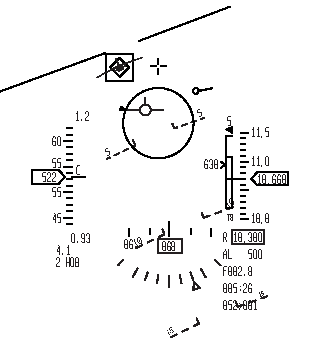
\includegraphics[
                height=75mm,
            ]{hud/aim9/full.pdf}
        };

        \node[
            draw,
            rounded 
            corners, 
            red, 
            minimum width=8.5mm, 
            minimum height=25mm
        ] (dlznode) at (12.5,1) {};

        % Annotations
        \node[lannot] (td) at ($(fig.west)+(-2.5mm,22.5mm)$) {Target designator box};
        \draw[->, red] (td.east) -- ++(25mm, 0mm);

        \node[lannot] (diamond) at ($(fig.west)+(-2.5mm,12.5mm)$) {Missile \\ diamond};
        \draw[->, red] (diamond.east) -- ++(18mm, 0mm) -- (-11mm, 21mm);

        \node[lannot] (weap) at ($(fig.west)+(-2.5mm,-19.5mm)$) {Selected weapon};
        \draw[->, red] (weap.east) -- ++(15mm, 0mm);

        \node[rannot] (cross) at ($(fig.east)+(2.5mm,34mm)$) {Boresight \\ cross};
        \draw[->, red] (cross.west) -- ++(-25mm, 0mm) -- (1mm, 24.5mm);

        \node[rannot] (ret) at ($(fig.east)+(2.5mm,24mm)$) {Missile \\ reticle};
        \draw[->, red] (ret.west) -- ++(-30mm, 0mm) -- (4mm, 19mm);

        \node[rannot] (dlz) at ($(fig.east)+(2.5mm,-15mm)$) {DLZ};
        \draw[->, red] (dlz.west) -- ++(-10mm, 0mm) -- (dlznode);
    \end{tikzpicture}
    \caption{AIM-9 HUD Symbology}
    \label{fig:aa_weap:aim9:hudsymb}
\end{figure}

\begin{figure}[htbp]
    \centering
    \begin{tikzpicture}[auto, node distance=10mm, x=1mm, y=1mm, very thick, line cap=round,
        >={Latex[round]}
        ]
        
        \node[draw, rounded corners] (fig) at (0,0) {
            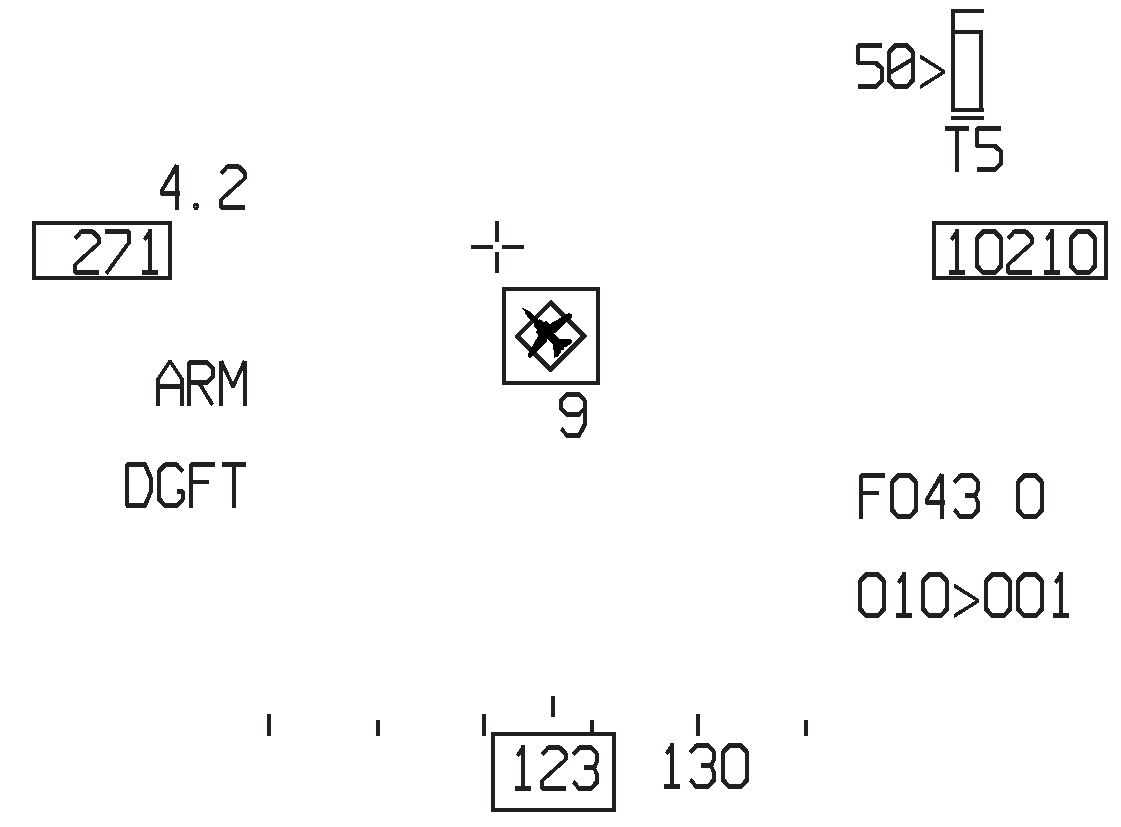
\includegraphics[
                height=50mm,
            ]{hmd/aim9_locked.pdf}
        };

        % Annotations
        \node[lannot] (diamond) at ($(fig.west)+(-2.5mm,20mm)$) {Boresight cross};
        \draw[->, red] (diamond.east) -- ++(20mm, 0mm) -- (-5.5mm, 11.5mm);

        \node[lannot] (td) at ($(fig.west)+(-2.5mm,5mm)$) {Target designator box};
        \draw[->, red] (td.east) -- ++(33mm, 0mm);

        \node[lannot] (mode) at ($(fig.west)+(-2.5mm,-10mm)$) {Mode};
        \draw[->, red] (mode.east) -- ++(7.5mm, 0mm) -- (-27mm, -7mm);

        \node[rannot] (dlz) at ($(fig.east)+(2.5mm,20mm)$) {DLZ};
        \draw[->, red] (dlz.west) -- ++(-10mm, 0mm);

        \node[rannot] (diamond) at ($(fig.east)+(2.5mm,0mm)$) {Missile \\ diamond};
        \draw[->, red] (diamond.west) -- ++(-32mm, 0mm) -- (1.5mm, 3mm);
    \end{tikzpicture}
    \caption{AIM-9 HMD Symbology}
    \label{fig:aa_weap:aim9:hmdsymb}
\end{figure}

\marginfigeometry

\subsubsection{AIM-9 SELECTION}
\begin{checklistitemize}
    \blueitem{Via DGFT}{(AIM-9 selected automatically)
    \begin{subenumerate}
        \item \textbf{DGFT/MSL OVRD} \dotfill \textbf{DGFT}
    \end{subenumerate}}
    \blueitem{Via MSL OVRD}{
    \begin{subenumerate}
        \item \textbf{DGFT/MSL OVRD} \dotfill \textbf{MSL OVRD}
        \item \textbf{Selected Weapon} \dotfill \textbf{9M/9X}
        \begin{itemize}
            \item \textbf{SMS OSB 7} --- \textbf{Press}
            \item or \textbf{NWS/MSL STEP} --- \textbf{Press (long)}
        \end{itemize}
    \end{subenumerate}}
    \blueitem{Via A-A Master Mode}{
    \begin{subenumerate}
        \item \textbf{Master Mode} \dotfill \textbf{A-A}
        \item \textbf{SMS OSB 1} \dotfill \textbf{Verify AAM} (default)
        \item \textbf{Selected Weapon} \dotfill \textbf{9M/9X}
        \begin{itemize}
            \item \textbf{SMS OSB 7} --- \textbf{Press}
            \item or \textbf{NWS/MSL STEP} --- \textbf{Press (long)}
        \end{itemize}
    \end{subenumerate}}
\end{checklistitemize}

\subsubsection{BORE EMPLOYMENT --- NO RADAR}
\label{subsec:aim9:bore}
\begin{checklistenumerate}
    \blueitem{Prerequisites}{
    \begin{subitemize}
        \item \textbf{RF Switch} \dotfill \textbf{SILENT} \\
        \hfill (if desired, completely silences radar)
        \item \textbf{Selected Weapon} \dotfill \textbf{9M/9X}
        \item \textbf{SLAVE/BORE} \dotfill \textbf{BORE}
        \item \textbf{WARM/COOL} \dotfill Verify \textbf{COOL}
        \item \textbf{Master Arm} \dotfill \textbf{ARM}
    \end{subitemize}}
    \blueitem{AIM-9 Track Acquisition}{
    \marginpar{
        \captionsetup{type=figure}
        \centering
        \begin{tikzpicture}[figstyle]
            \node[boxedmarfigstyle] (fig) at (0,0) {
                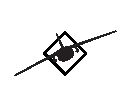
\includegraphics[
                    scale=1.25,
                ]{hud/aim9/subfig_missile_diamond.pdf}
            };
        \end{tikzpicture}
        \caption{AIM-9 missile diamond latched to target, indicating lock.}
    }
    \begin{subenumerate}
        \item \textbf{Missile Reticle} \dotfill \textbf{On-Target}
        \item \textbf{Sidewinder Audio} \dotfill \textbf{Lock Tone}
        \item \textbf{CAGE/UNCAGE} \dotfill \textbf{Press}
        \item \textbf{Missile Diamond} \dotfill verify latched to target
    \end{subenumerate}}
    \blueitem{Fire Missile}{
    \begin{subenumerate}
        \item Maneuver into firing position
        \item \textbf{Sidewinder Audio} \dotfill \textbf{Lock Tone}
        \item \textbf{WPN REL} \dotfill \textbf{Depress}
    \end{subenumerate}}
\end{checklistenumerate}

\clearpage

\subsubsection{HMCS BORE EMPLOYMENT --- NO RADAR}
\label{subsec:aim9:hmcs}
\begin{checklistenumerate}
    \blueitem{Prerequisites}{
    \begin{subitemize}
        \item \textbf{HMD SYMB. INT} \dotfill \textbf{INT}
        \item \textbf{RF Switch} \dotfill \textbf{SILENT} \\
        \hfill (if desired, completely silences radar)
        \item \textbf{Selected Weapon} \dotfill \textbf{9M/9X}
        \item \textbf{SLAVE/BORE} \dotfill \textbf{BORE}
        \item \textbf{WARM/COOL} \dotfill Verify \textbf{COOL}
        \item \textbf{Master Arm} \dotfill \textbf{ARM}
    \end{subitemize}}
    \blueitem{AIM-9 Track Acquisition}{
    \marginpar{
        \captionsetup{type=figure}
        \begin{tikzpicture}[figstyle]
            \node[boxedmarfigstyle] (fig) at (0,0) {
                
\includegraphics[
                    scale=0.75,
                ]{hmd/aiming_cross.pdf}
            };
        \end{tikzpicture}
        \caption{AIM-9 seeker follows HMD aiming cross}
    }
    \marginpar{
        \captionsetup{type=figure}
        \begin{tikzpicture}[figstyle]
            \node[boxedmarfigstyle] (fig) at (0,0) {
                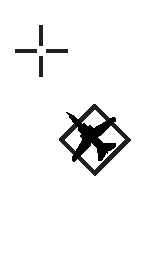
\includegraphics[
                    scale=0.5,
                ]{hmd/aim9_track_missile_diamond.pdf}
            };
        \end{tikzpicture}
        \caption{AIM-9 HMD track}
    }
    \marginpar{
        \captionsetup{type=figure}
        \begin{tikzpicture}[figstyle]
            \node[boxedmarfigstyle] (fig) at (0,0) {
                
\includegraphics[
                    scale=0.75,
                ]{hmd/los.pdf}
            };
        \end{tikzpicture}
        \caption{X indicates HMD beyond AIM-9 seeker limits}
    }
    \begin{subenumerate}
        \item Maneuver to place target within AIM-9 seeker limits
        \item \textbf{HMD Aiming Cross} \dotfill \textbf{On-Target}
    \end{subenumerate}

    Missile diamond follows aiming cross (within seeker limits)

    \begin{subenumerate}[start=3]
        \item \textbf{Sidewinder Audio} \dotfill \textbf{Lock Tone}
        \item \textbf{CAGE/UNCAGE} \dotfill \textbf{Press}
        \item \textbf{Missile Diamond} \dotfill verify latched to target
    \end{subenumerate}}
    \blueitem{Fire Missile}{
    \begin{subenumerate}
        \item Maneuver into firing position
        \item \textbf{Sidewinder Audio} \dotfill \textbf{Lock Tone}
        \item \textbf{WPN REL} \dotfill \textbf{Depress}
    \end{subenumerate}}
\end{checklistenumerate}

\clearpage

\subsubsection{SLAVE EMPLOYMENT --- RADAR}
\label{subsec:aim9:slave}
\begin{checklistenumerate}
    \blueitem{Prerequisites}{
    \begin{subitemize}
        \item \textbf{FCR Switch} \dotfill \textbf{FCR}
        \item \textbf{RF Switch} \dotfill \textbf{NORM}
        \item \textbf{HMD SYMB. INT} \dotfill As desired
        \item \textbf{Selected Weapon} \dotfill \textbf{9M/9X}
        \item \textbf{SLAVE/BORE} \dotfill Verify \textbf{SLAVE}
        \item \textbf{WARM/COOL} \dotfill Verify \textbf{COOL}
        \item \textbf{Master Arm} \dotfill \textbf{ARM}
    \end{subitemize}}
    \blueitem{Radar Acquisition}{ACM selected automatically in \textbf{DGFT} mode, \textbf{see \Cref{subsec:acm}}
    \marginpar{
        \captionsetup{type=figure}
        \centering
        \begin{tikzpicture}[figstyle]

            % \draw[color2, fill=color2!20, dashed] 
            % (0,-6) circle [x radius=8, y radius=11.5];
            
            \node[boxedmarfigstyle] (bore) at (0,0) {
                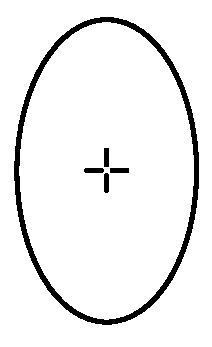
\includegraphics[
                    scale=0.5,
                ]{hmd/dgft_subfig_bore.pdf}
            };
        \end{tikzpicture}
        \caption{HMD BORE scan zone}
    }
    
    \medskip
    For demonstration we will use \textbf{ACM BORE Submode} with HMD
    
    \begin{subenumerate}
        \item \textbf{FCR Mode} \dotfill \textbf{ACM}
        \item \textbf{TMS} \dotfill \textbf{FWD}
        \item \textbf{Target} \dotfill \textbf{In HMD BORE Symbol}
        \item \textbf{Radar} \dotfill wait for \textbf{STT Lock}
    \end{subenumerate}
    
    Can also lock from CRM, \textbf{see \Cref{subsec:crm}}
    }
    \blueitem{AIM-9 Track Acquisition}{
    \marginpar{
        \captionsetup{type=figure}
        \centering
        \begin{tikzpicture}[figstyle]
            \node[boxedmarfigstyle] (fig) at (0,0) {
                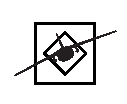
\includegraphics[
                    scale=1.25,
                ]{hud/aim9/subfig_td_box_missile_diamond.pdf}
            };
        \end{tikzpicture}
        \caption{AIM-9 missile diamond and target designator box latched to target, indicating radar and seeker lock.}
    }
    \begin{subenumerate}
        \item \textbf{CAGE/UNCAGE} \dotfill \textbf{Press}
        \item \textbf{Sidewinder Audio} \dotfill \textbf{Lock Tone}
        \item \textbf{Missile Diamond} \dotfill verify latched to target
    \end{subenumerate}}
    \blueitem{Fire Missile}{
    \marginpar{
        \captionsetup{type=figure}
        \centering
        \begin{tikzpicture}[figstyle]
            \node[boxedmarfigstyle] (fig) at (0,0) {
                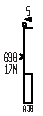
\includegraphics[
                    scale=2.5,
                ]{hud/aim9/subfig_dlz.pdf}
            };
        \end{tikzpicture}
        \caption{In-range DLZ}
    }
    \begin{subenumerate}
        \item Maneuver into firing position
        \item \textbf{DLZ} \dotfill indicates \textbf{In-Range}
        \item \textbf{Sidewinder Audio} \dotfill \textbf{Lock Tone}
        \item \textbf{WPN REL} \dotfill \textbf{Depress}
    \end{subenumerate}}
\end{checklistenumerate}

\marginfigrestore 